\documentclass[aspectratio = 169]{beamer}
\usetheme{OsloMet}
\setbeamersize{text margin left=0.5cm,text margin right=0.5cm}
\usepackage{style}
\usepackage{subfig}
\usepackage{xcolor}
\usepackage{hyperref}
\renewcommand{\S}{\mathcal{S}}
\newcommand{\T}{\mathcal{T}}
\author[]{Mahsa Azizi, Erik Chan\\ Xilai Fu, Nima Safaian\\ S. Parisa Torabi, Wenning Wei}
\title{Modeling Canadian\\ Heavy Crude\\ Congestion Pricing}


\begin{document}

\begin{frame}{OUTLINE}
\begin{enumerate}
\setlength\itemsep{2em}
    \item\Large{Introduction}
    \item Model
    \item Result
    \item Future work
\end{enumerate}
\end{frame}

\section{Introduction}
\begin{frame}{Introduction-Spatial price integration}

\begin{itemize}
\setlength\itemsep{2em}
    \item \Large{Crude oil classification: Lighter oils are higher in price due to an easier \&  cheaper process in refineries rather than heavy oils }
    \item \Large{Location of extraction: It needs to be transported to the point of refinery}
    \item \Large{Transportation capacity: Type of transportation and their capacitance, either pipelines or trains}

\end{itemize}
\end{frame}




\begin{frame}{Introduction - Oil price benchmarks}
    \begin{itemize}
\setlength\itemsep{2em}
    \item \Large{West Texas Intermediate(WTI)}
    \item \Large{West Canada Select (WCS)}
    %Is this relevant.
    \item Alberta produces 4MM barrels per day. Two-thirds of the WCS production is consumed in United States.
    \item The spread between WTI and WCS is estimated about \$5 US due to the different oil classification
\end{itemize}
\end{frame}

%These figures need to be as large as possible to prevent the content from being clipped.
%Do not titles to frames like this - it already has a title in the figure.
\begin{frame}{}

\centering
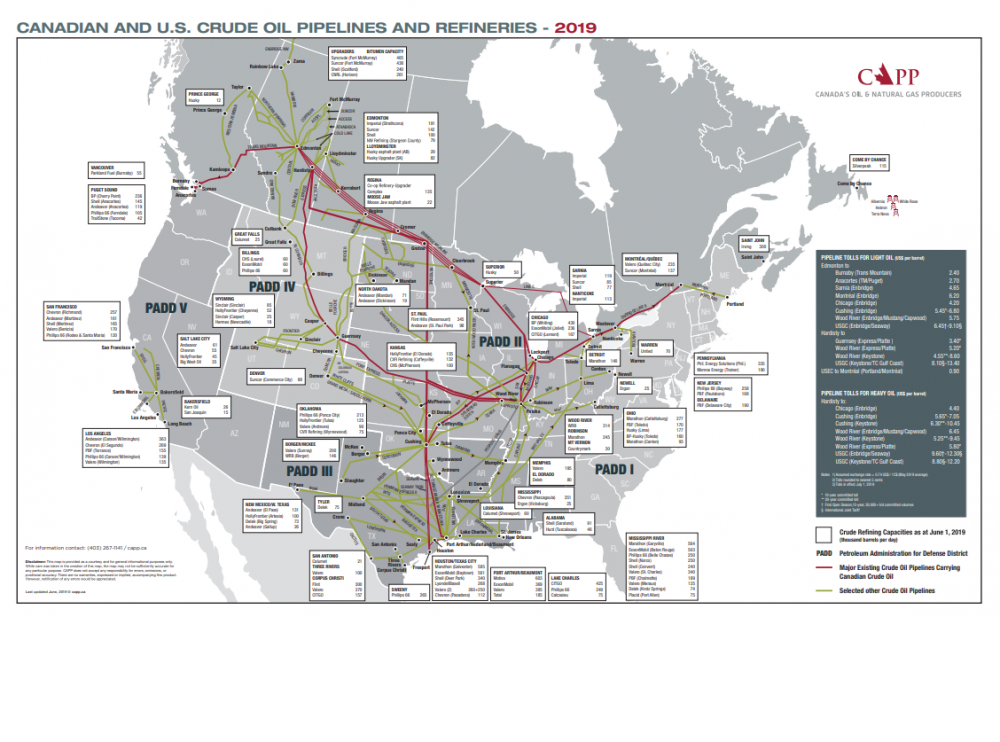
\includegraphics[scale=0.50]{OM-images/piplines.png}

\end{frame}

%These figures need to be as large as possible to prevent the content from being clipped.
%Do not titles to frames like this - it already has a title in the figure.
\begin{frame}{}
 \begin{figure}
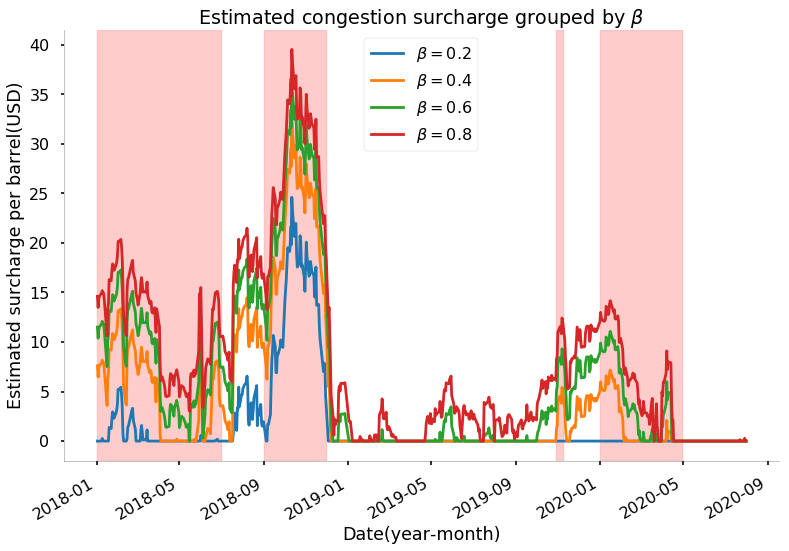
\includegraphics[scale = 0.40]{image.png}
\end{figure}
\end{frame}

\begin{frame}{Model - Price decomposition of the spread}
This model is based off of the work of Birge et al., \emph{Spatial price integration in commodity markets with capacitated transportation networks}, 2020.
\vspace{0.5cm}

For a network with fixed costs and fixed network structure, we decompose the equilibrium of the WTI--WCS price spread $\lambda^{t}$ as follows:
    \[\lambda^{t} = \rho + \varepsilon^{t} + \omega^{t}\]
where
\begin{enumerate}
    \item $\lambda^{t}$: the WTI--WCS price spread at time $t$;
    \item $\rho$: the transportation cost;
    \item $\varepsilon^{t}$: a baseline equilibrium value;
    \item $\omega^{t}$: the congestion surcharge at time $t$.
\end{enumerate}
\end{frame}

\begin{frame}{Model - The neutral band}
\begin{alertblock}{Uniqueness}
{In general, equilibrium prices are NOT unique in a transportation network.}\end{alertblock}
\begin{example}
The price of a bottle of olive oil is \$15 in Vancouver (YVR) and \$20 in Calgary (YYC). It costs \$8 to transport each bottle between YVR and YYC.
\end{example}
Is there arbitrage? 
\end{frame}

\begin{frame}{Model - The neutral band}
\begin{alertblock}{Uniqueness}
{In general, equilibrium prices are NOT unique in a transportation network.}\end{alertblock}
\begin{example}
The price of a bottle of olive oil is \$15 in Vancouver (YVR) and \$20 in Calgary (YYC). It costs \$8 to transport each bottle between YVR and YYC.
\end{example}
Is there arbitrage?

No. For any price at YVR in the interval [\$12, \$28] and there will be no arbitrage. We call this the \emph{neutral band}.
\end{frame}

\begin{frame}{Model - A one node model}
\begin{align*}
\text{minimize: } &\alpha\\\label{2}
\text{subject to: } &\lambda^t = \rho + \varepsilon^t +\omega^t, \quad \forall t\in\T,\\
&-\alpha\leq\varepsilon^t \leq \alpha,\quad \forall t\in \T\\
&0\leq\omega^t\leq \psi^t M,\quad \forall t\in\T\\
&\varepsilon^t \geq \alpha - (1-\psi^t) M,\quad \forall t\in \T\\
&\sum_t \psi^t \leq \beta T,\\
&\psi^t \in\{0,1\}, \quad \forall t\in \T.
\end{align*}

Here $\beta$ and $M$ are constants where $\beta \in [0,1]$ and $M$ is a sufficiently large upper bound for congestion.
\end{frame}

\begin{frame}{}
\centering
\vspace{-0.5cm}
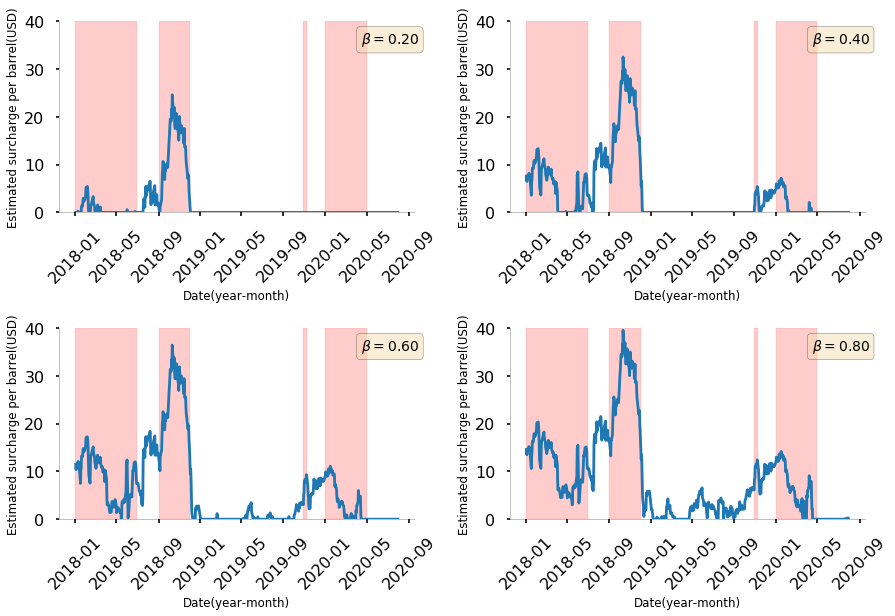
\includegraphics[scale = 0.4]{image3.png}
\end{frame}

\begin{frame}{Model - A multi-node model}
\vspace{-0.7cm}
\begin{figure}
%\footnotesize
\begin{equation*}
\begin{split}
\text{minimize: } &\sum_{s\in\S} \alpha_s\\
\text{subject to: } &\lambda_s^t = \rho_s + \varepsilon_s^t +\omega_s^t, \quad \forall s\in\S,~\forall t\in\T,\\
&-\alpha_s\leq\varepsilon_s^t \leq \alpha_s,\\
&0\leq\omega_s^t\leq \psi^t M,\\
&\varepsilon_s^t \geq \alpha_s - (1-\gamma_s^t) M,\\
&\psi^t \leq \sum_s \gamma_s^t\leq |S|\,\psi^t,\\
&\sum_t \psi^t \leq \beta T,\\
&\psi^t, \gamma_s^t \in\{0,1\},
\end{split}
\end{equation*}
\end{figure}
Here $\beta$ and $M$ are constants where $\beta \in [0,1]$ and $M$ is a sufficiently large upper bound for congestion, and $\lvert \cdot \rvert$ denotes the cardinality of a set.
\end{frame} 


\begin{frame}{Model - Ornstein--Uhlenbeck process}
$$\operatorname{d}\!S_t = \alpha(\mu-S_t)\,\operatorname{d}\!t +\sigma \,\operatorname{d}\!W_t$$
\bigskip
The SDE is calibrated to the WTI/WCS spread with parameters: 
$$\alpha = 0.0119, \quad \mu = 16.3,\quad\sigma = 1.45.$$
We simulate three paths using the correlation matrix:
%\begin{equation*}
%\left[
%\begin{array}{lr}
%             &~1~~~~~0.8~~~~~0.7\\
%             &0.8~~~~1~~ ~~0.56\\
%            & 0.7~~~~0.56~~~~~1 
%             \end{array}
%\right].
%\end{equation*}
\begin{equation*}\operatorname{corr} = 
    \begin{bmatrix}
    1& 0.8& 0.7\\
    0.8& 1 &0.56\\
    0.7 & 0.56 &1
    \end{bmatrix}
\end{equation*}
\end{frame}


\begin{frame}{Simulated paths of the spread}
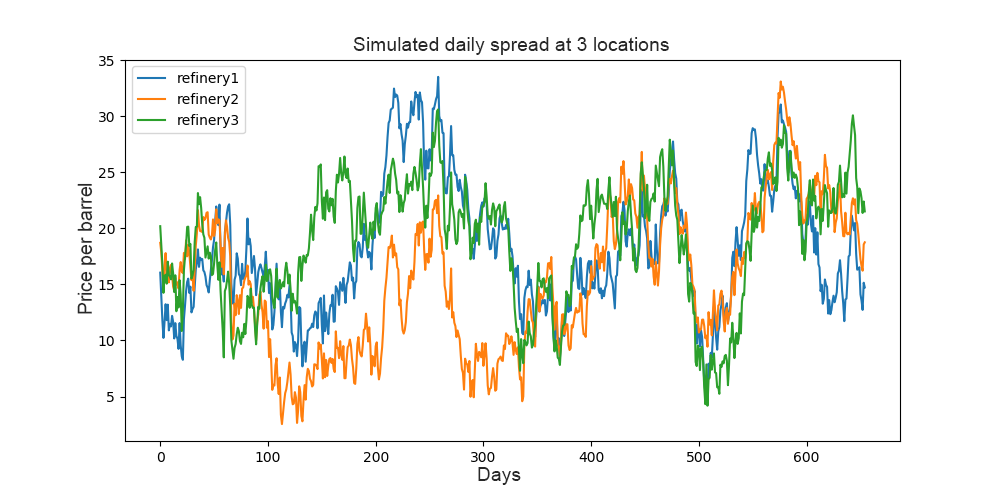
\includegraphics[width=\linewidth]{simulated spread (1).png}
\end{frame}


%\begin{frame}{Estimated congestion surcharge for $\beta = 0.4$}
%\begin{figure}
%   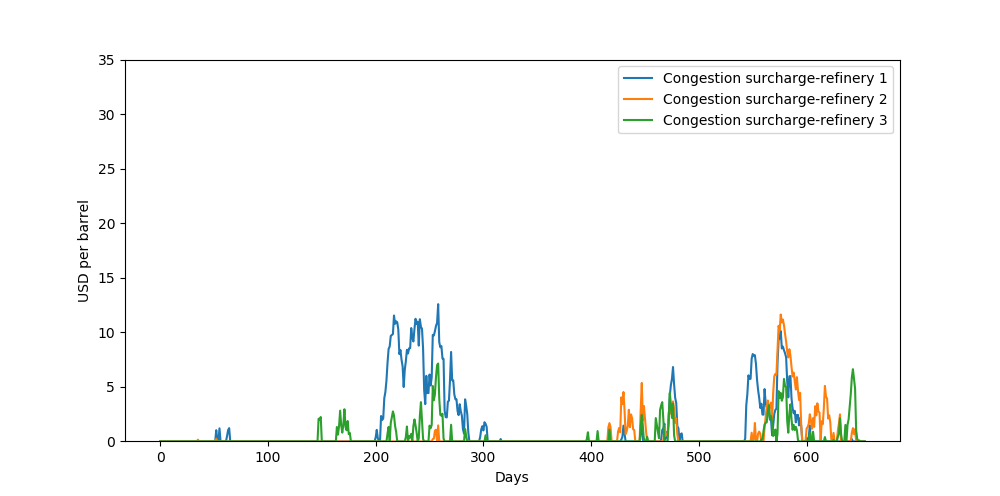
\includegraphics[scale = 0.55]{3node_beta.4.png}
%\end{figure}
%\end{frame}

\begin{frame}{Estimated congestion surcharge for $\beta = 0.6$}
\begin{figure}
    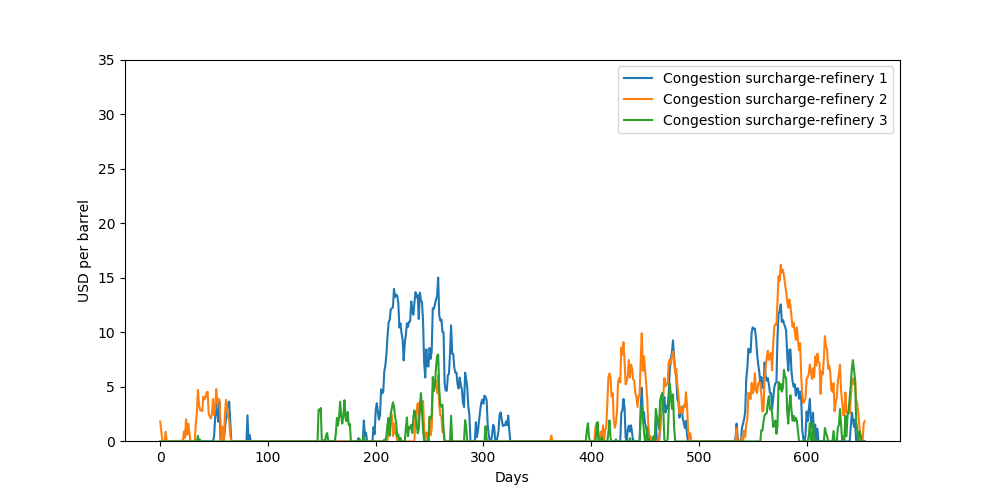
\includegraphics[scale = 0.55]{3node_beta.6.png}
\end{figure}
\end{frame}


\begin{frame}[c]{}
    \begin{center}
        \huge{Thank you for your attention.}
    \end{center}
\end{frame}

\end{document}